\documentclass[11pt,a4paper]{article}\usepackage[utf8]{inputenc}

\usepackage[T1]{fontenc}
\usepackage{tgpagella}
\usepackage[spanish]{babel}
\usepackage{geometry}
\usepackage{graphicx}
\usepackage{booktabs}
\usepackage{array}
\usepackage{xcolor}
\usepackage{titlesec}
\usepackage{fancyhdr}
\usepackage[parfill]{parskip}
\usepackage[expansion=false]{microtype}
\usepackage{hyperref}
\usepackage{setspace}
\usepackage{needspace}

\geometry{top=3.0cm,bottom=3.0cm,left=3.5cm,right=3.5cm}
\setlength{\parskip}{0.65em}
\setlength{\parindent}{0em}

\definecolor{azulai}{RGB}{30,80,140}
\definecolor{doradoai}{RGB}{140,90,0}
\definecolor{grisai}{RGB}{70,70,70}

\titleformat{\section}{\Large\bfseries\color{azulai}}{}{0em}{}[{\color{azulai}\titlerule[0.5pt]\nopagebreak[4]}]
\titlespacing*{\section}{0pt}{1.8em}{0.8em}
\titleformat{\subsection}{\large\bfseries\color{doradoai}}{}{0em}{}[{\nopagebreak[4]}]
\titlespacing*{\subsection}{0pt}{1.4em}{0.5em}
\titleformat{\subsubsection}{\normalsize\bfseries\color{grisai}}{}{0em}{}[{\nopagebreak[4]}]
\titlespacing*{\subsubsection}{0pt}{1.0em}{0.3em}

\pagestyle{fancy}\fancyhf{}
\rhead{\textcolor{grisai}{\small Amaya Beatriz — Arquitectura Interna}}
\lhead{\textcolor{grisai}{\small Carta Natal Completa}}
\cfoot{\textcolor{grisai}{\small\thepage}}
\renewcommand{\headrulewidth}{0.3pt}

\hypersetup{colorlinks=true,linkcolor=azulai,urlcolor=azulai}
\setstretch{1.45}
\tolerance=1500
\emergencystretch=4em

\begin{document}

% ── Portada ──────────────────────────────────────────────────────────────────
\begin{titlepage}
  \centering
  \vspace*{1.5cm}
  {\Huge\bfseries\color{azulai} Carta Natal Completa}\\[0.5cm]
  {\large\color{grisai} Arquitectura Interna}\\[0.3cm]
  {\small\itshape\color{grisai} Un método para sostener cuerpo, energía y vida con coherencia}\\[2cm]
  {\huge\color{doradoai} Amaya Beatriz}\\[1.5cm]
  {\Large 30/10/1976 \quad 22:10}\\[0.3cm]
  {\Large Zaragoza, España}\\[0.3cm]
  {\normalsize Lat: 41.6916° \quad Lon: -0.9101° \quad UTC+01:00}\\[0.3cm]
  {\normalsize Ascendente: Cáncer 16°08' \quad
    MC: Piscis 25°32'}\\[2.5cm]
  \vfill
  {\small Generado el 19/05/2026}
\end{titlepage}

\tableofcontents
\newpage

% ── Rueda ─────────────────────────────────────────────────────────────────────
\section{Carta Natal}
\begin{figure}[h!]
  \centering
  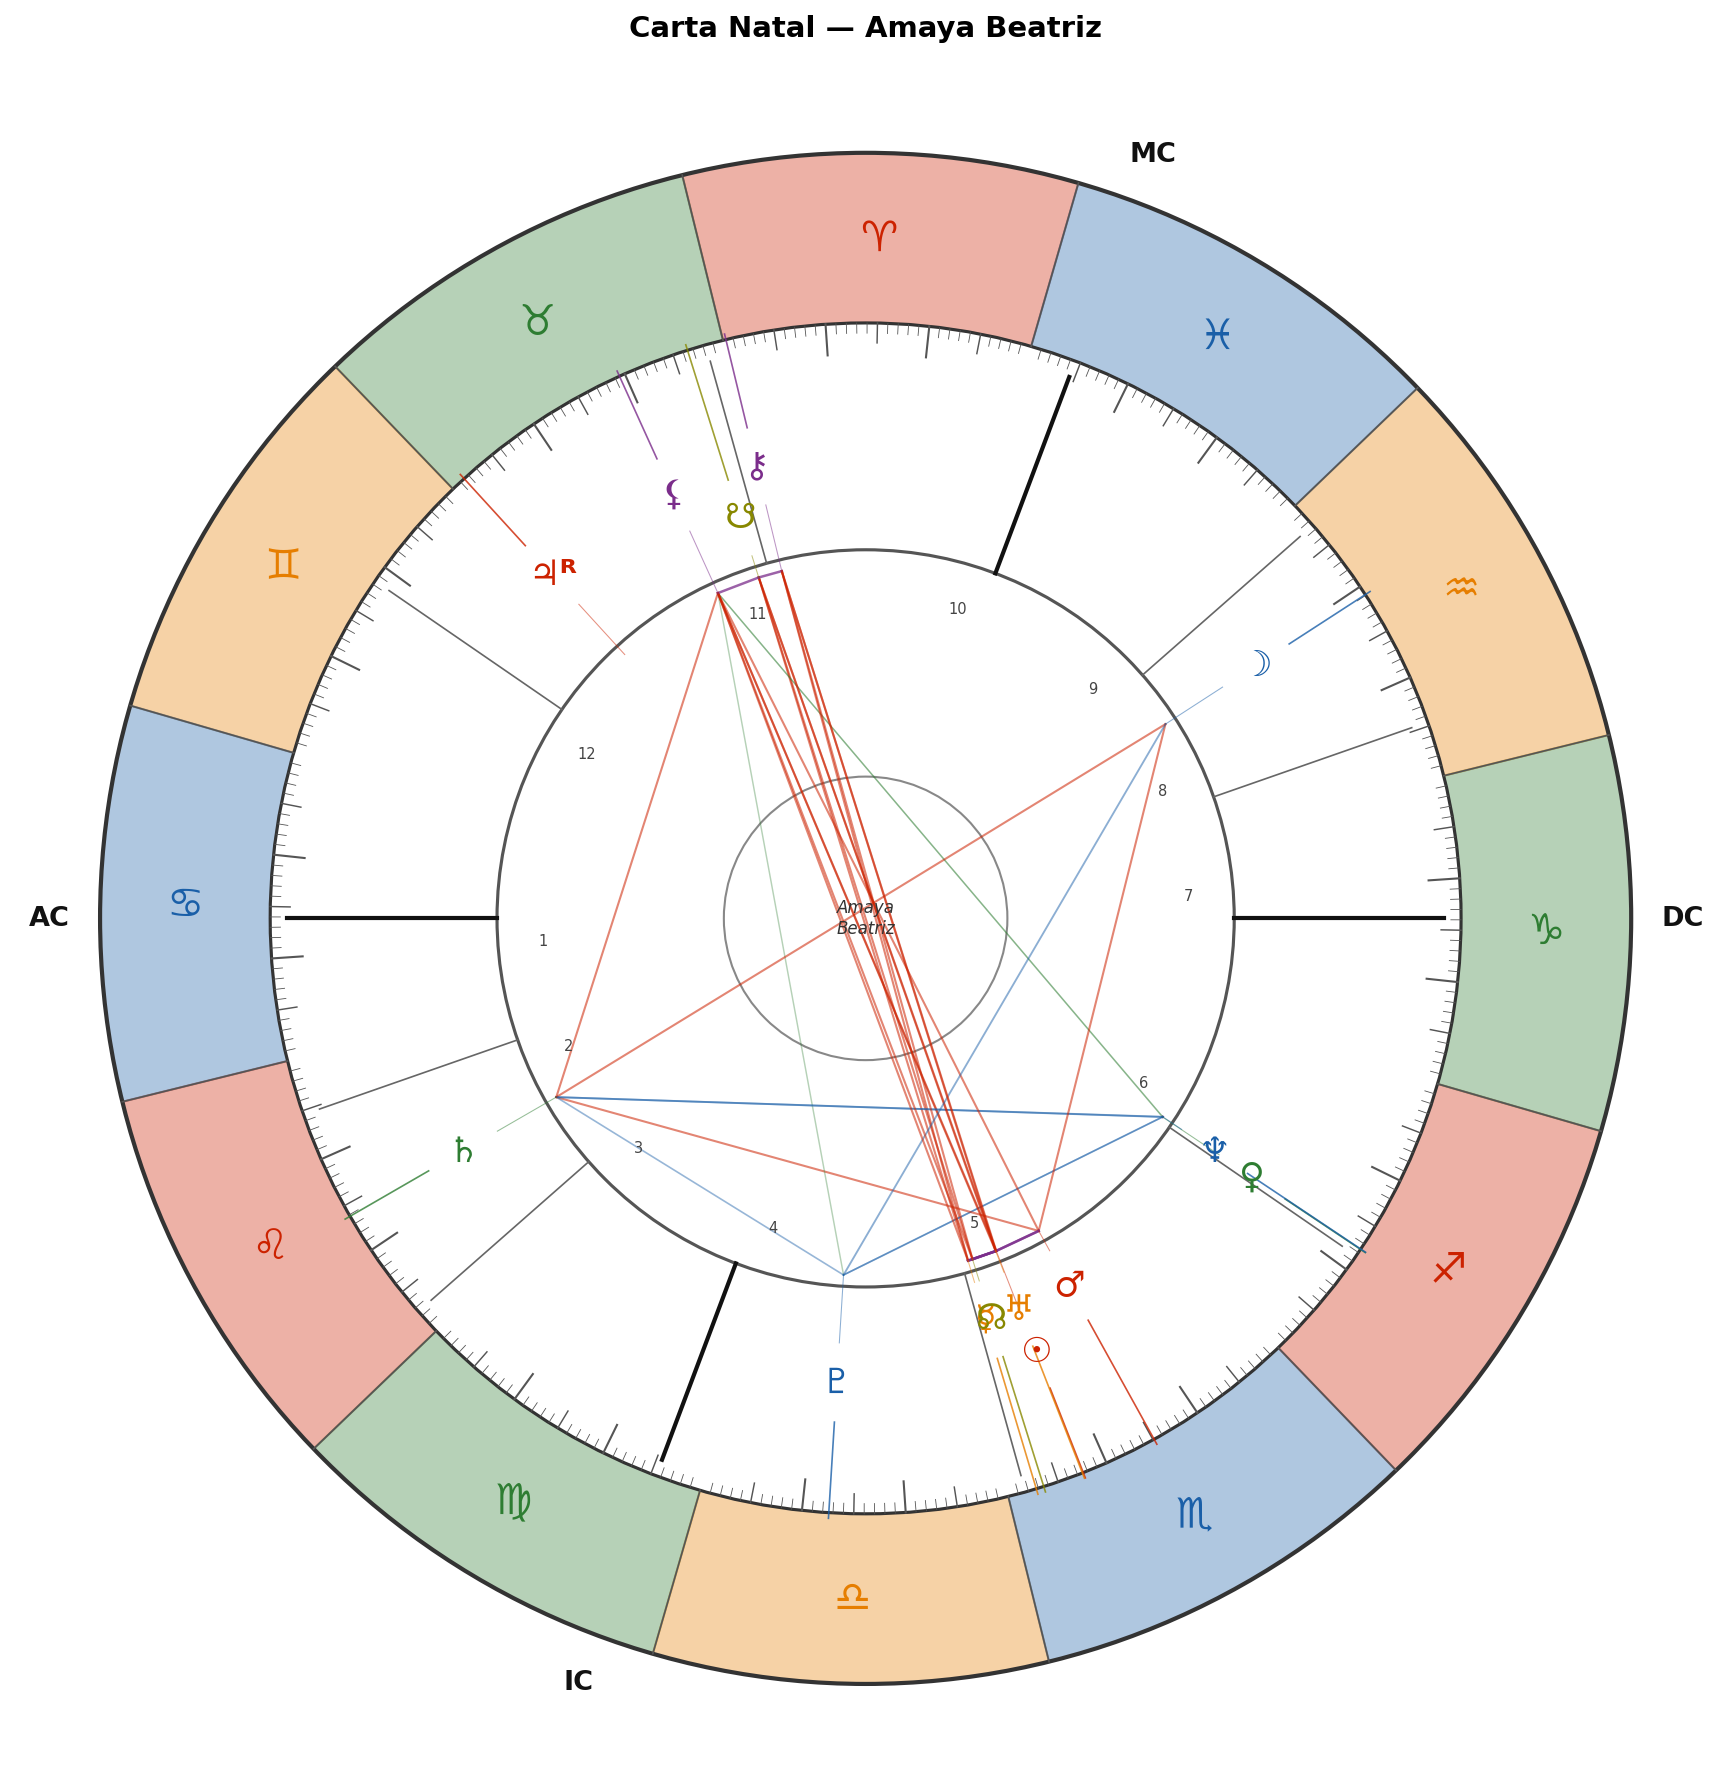
\includegraphics[width=0.90\textwidth]{Amaya_Beatriz_AI_rueda.png}
  \caption{Carta natal de Amaya Beatriz — 30/10/1976 22:10 — Zaragoza, España}
\end{figure}

\newpage

% ── Tabla de posiciones ───────────────────────────────────────────────────────
\section{Posiciones Planetarias}

\begin{center}
\begin{tabular}{llrrlll}
  \toprule
  \textbf{Planeta} & \textbf{Signo} & \textbf{Grado} & \textbf{Casa} &
  \textbf{Elemento} & \textbf{R} \\
  \midrule
  Sol & Escorpio & 7°35' & 5 & Agua &  \\
  Luna & Acuario & 19°05' & 8 & Aire &  \\
  Mercurio & Escorpio & 2°48' & 5 & Agua &  \\
  Venus & Sagitario & 12°22' & 6 & Fuego &  \\
  Marte & Escorpio & 15°07' & 5 & Agua &  \\
  Júpiter & Tauro & 28°32' & 11 & Tierra & R \\
  Saturno & Leo & 16°10' & 2 & Fuego &  \\
  Urano & Escorpio & 7°29' & 5 & Agua &  \\
  Neptuno & Sagitario & 12°24' & 6 & Fuego &  \\
  Plutón & Libra* & 12°36' & 4 & Aire &  \\
  Quirón & Aries* & 29°43' & 10 & Fuego &  \\
  Lilith & Tauro & 10°34' & 11 & Tierra &  \\
  Nodo Norte & Escorpio & 3°33' & 5 & Agua &  \\
  Nodo Sur & Tauro & 3°33' & 11 & Tierra &  \\
  \bottomrule
\end{tabular}
\end{center}

\vspace{0.5cm}
\begin{itemize}
  \item \textbf{Ascendente:} Cáncer 16°08'
  \item \textbf{Medio Cielo:} Piscis 25°32'
  \item \textbf{Signos interceptados} (marcados con * en la tabla):
  \begin{itemize}
  \item Aries (casa 10) -- Libra (casa 4)
  \end{itemize}
\end{itemize}

\newpage

% ── Interpretación ────────────────────────────────────────────────────────────
\section{Interpretación — Arquitectura Interna}

\begin{center}
{\small\itshape
No se trata de definirte. Se trata de observar cómo se organiza tu energía,\
dónde puedes perder equilibrio y qué apoyos te ayudan a sostenerte.
}
\end{center}

\vspace{0.5cm}

\subsection{1. Visión General}

Tu carta muestra la siguiente distribución de elementos: Fuego 3.5, Tierra 1, Aire 4, Agua 8. Agua (profundidad emocional, capacidad de resonancia, sensibilidad abierta): ahí está el peso de tu carta. Es el registro desde el que tu energía se activa con más fluidez y sin esfuerzo consciente. Tierra (arraigo en lo concreto, estructura material, ritmo sostenido y contacto con el cuerpo) está poco representado en tu carta. Ese territorio puede pedirte un esfuerzo consciente, especialmente cuando la presión sube. La mayoría de tus planetas están en signos fijos: hay capacidad de persistencia, estabilidad y continuidad. Cuando algo tiene sentido para ti, puedes sostenerlo durante mucho tiempo incluso en condiciones difíciles. La dificultad aparece cuando hace falta cambiar de dirección y una parte de ti sigue intentando mantener lo conocido. Tu Medio Cielo en Piscis: La creatividad, la sensibilidad hacia el entorno y la capacidad de adaptarte a distintos contextos humanos. Funcionas bien en espacios donde hace falta imaginación, escucha o flexibilidad.

\vspace{0.8cm}
\Needspace{5\baselineskip}

\subsection{2. Ejes Principales}

\subsubsection*{Sol en Escorpio — Casa 5}
Tu Sol en Escorpio funciona con intensidad y necesidad de implicación real. No te resulta fácil hacer las cosas a medias ni permanecer mucho tiempo en situaciones que sientes vacías o superficiales. Cuando algo importa, tiendes a implicarte profundamente y a percibir rápidamente las tensiones ocultas. El riesgo aparece cuando la necesidad de protegerte te lleva a controlar demasiado o a cerrarte antes de tiempo. En Casa 5, la creatividad, el juego y la expresión auténtica son dimensiones estructurales de tu identidad. Necesitas crear algo que lleve tu marca. Sin espacios de expresión genuina, puedes apagarte o perder motivación.

\subsubsection*{Luna en Acuario — Casa 8}
Tu Luna en Acuario necesita espacio emocional y cierta distancia para procesar lo que siente. Cuando las emociones son demasiado intensas o invasivas, puedes retirarte o irte rápidamente a la cabeza para intentar entenderlas. La libertad dentro de los vínculos es importante para que puedas sentirte bien emocionalmente. Cuando sientes demasiada presión emocional, aparece necesidad de alejarte o desconectarte. En Casa 8, las emociones suelen vivirse con intensidad y profundidad aunque no siempre se expresen fácilmente. Los vínculos importantes, las pérdidas o las situaciones límite tienden a afectarte mucho más de lo que parece desde fuera. Cuando algo te toca emocionalmente, no te resulta fácil quedarte en la superficie.

\subsubsection*{Ascendente Cáncer}
Tu Ascendente en Cáncer hace que te presentes ante los demás de forma receptiva, empática y algo protectora. Tienes una sensibilidad de fondo que observa el entorno emocional antes de abrirte. Tu primera impresión puede ser de suavidad o de reserva, según el contexto. Su regente es la Luna, en Acuario y Casa 8. El Ascendente toma el tono de Acuario: independiente, analítica y poco convencional. Esa energía opera principalmente desde los vínculos intensos, las pérdidas y las situaciones difíciles de controlar.

\subsubsection*{Grados finales de signo}
Los grados finales de signo suelen hablar de zonas de la carta donde hay mucha experiencia acumulada y sensación de       cierre de etapa. La energía no se vive de forma ligera o automática: suele haber más intensidad, más consciencia y la sensación de que una forma antigua de funcionar ya no termina de encajar igual.

No significa algo negativo ni indica un destino fijo. Simplemente muestra lugares donde la vida suele pedir más presencia, más maduración y una manera distinta de responder.

En esta carta aparecen posiciones en grado anarético (29°). Estos grados suelen sentirse como puntos de máxima intensidad dentro de un signo. Hay mucha experiencia acumulada, pero también sensación de presión interna, cansancio de repetir ciertos patrones o necesidad de cambio.

A veces se vive como si ya no fuera posible seguir respondiendo exactamente igual que antes.

Quirón en Aries 29°43', Casa 10 aparece en grado anarético. Hay una zona especialmente sensible en tu vida que puede sentirse vulnerable o expuesta desde hace mucho tiempo. Esa sensibilidad puede doler, pero también darte una capacidad muy profunda para comprender procesos similares en otras personas. No se trata de eliminar esa parte de ti, sino de dejar de vivirla como un defecto.

También aparecen posiciones en grados previos al anarético. No suelen sentirse tan extremos como el grado 29, pero sí muestran zonas donde ya existe bastante maduración y donde empiezan a aparecer señales de cambio o agotamiento de una forma antigua de funcionar.

Júpiter en Tauro 28°32', Casa 11 aparece en grado previo al anarético. La necesidad de crecer, expandirte y encontrar sentido aparece con mucha fuerza. Puede costarte permanecer mucho tiempo en experiencias que sientes pequeñas, limitadas o vacías de propósito. A veces puedes buscar siempre el siguiente horizonte antes de terminar de integrar lo que ya estás viviendo. El aprendizaje está en encontrar amplitud sin perder estabilidad.

Cuando varios puntos de la carta están al final de signo, la vida puede sentirse más intensa o vivirse con menos sensación de margen interno. A veces aparece urgencia, cansancio de ciertas dinámicas o sensación de estar cerca de cambios importantes incluso aunque externamente todo siga igual.

No significa que la vida vaya a ser más difícil. Significa que esas zonas necesitan más consciencia, más pausa y una forma más presente de responder, en lugar de seguir funcionando únicamente desde hábitos automáticos.


\subsubsection*{Signos interceptados}
Los signos Aries (Casa 10) con Quirón y Libra (Casa 4) con Plutón aparecen interceptados: su expresión puede sentirse menos inmediata o menos natural al principio. Esto influye especialmente en Quirón, Plutón, que pueden necesitar más tiempo, experiencia o situaciones concretas para sentirse plenamente desarrollados. Muchas veces estas posiciones no se muestran rápido desde fuera, pero ganan fuerza y claridad con los años.

\vspace{0.8cm}
\Needspace{5\baselineskip}

\subsection{3. Organización de la Energía}

Tu Mercurio en Escorpio no se queda fácilmente en la superficie. Tiendes a buscar lo que hay detrás de las palabras, los silencios o las contradicciones. El riesgo aparece cuando la mente entra en sospecha o intensidad y le cuesta soltar una idea. En Casa 5, la mente necesita creatividad, expresión y cierta libertad para funcionar bien. Piensas mejor cuando hay entusiasmo, juego o posibilidad de poner algo personal en lo que haces. Tu Venus en Sagitario necesita libertad, movimiento y sentido compartido. El vínculo se fortalece cuando hay crecimiento, aprendizaje o una dirección que ilusiona. El riesgo aparece cuando cualquier límite se vive como encierro, incluso cuando el vínculo necesita estructura. En Casa 6, el afecto suele expresarse a través del cuidado cotidiano y los gestos prácticos. Estar pendiente de lo que hace falta puede ser una forma importante de mostrar amor. Tu Marte en Escorpio actúa con intensidad, resistencia y mucha concentración cuando algo importa. No se mueve de forma ligera: necesita implicación real. El riesgo aparece cuando la fuerza se convierte en control, tensión acumulada o dificultad para soltar una batalla. En Casa 5, la energía necesita creatividad, juego y emoción para activarse del todo. Funcionas mejor cuando puedes poner entusiasmo, deseo o expresión personal en lo que haces.

\vspace{0.8cm}
\Needspace{5\baselineskip}

\subsection{4. Estructura y Tensión}

\subsubsection*{Concentración de energía}

Hay una concentración notable en Casa 5: Sol, Mercurio, Marte, Urano y Nodo Norte. Cuando varios planetas ocupan la misma casa, esa área absorbe buena parte de la actividad vital. En esta carta, el foco de la creatividad, el disfrute y la expresión personal funciona como núcleo central: ahí se acumula la presión, la demanda es mayor y también hay más recursos disponibles para operar. No es necesariamente un conflicto, pero sí un punto de alta intensidad sostenida.

También hay una concentración significativa en Casa 11: Júpiter, Nodo Sur y Lilith. En este caso, el foco se desplaza hacia las amistades, los grupos y los proyectos compartidos. Es un ámbito donde la exigencia aumenta, donde se concentra parte de la presión y donde también existe capacidad real de sostener procesos importantes. Tampoco es en sí un problema, pero sí un área de intensidad mantenida.



Los aspectos aparecen organizados en dos niveles. Los aspectos exactos (orbe igual o menor a 1°) suelen sentirse de forma más inmediata y constante en la vida cotidiana. Los aspectos estructurales tienen un orbe más amplio, pero siguen describiendo dinámicas importantes que se repiten a lo largo de la vida.



\vspace{0.8cm}
\Needspace{5\baselineskip}
\subsubsection*{Aspectos exactos}
\Needspace{3\baselineskip}
\subsubsection*{Venus (Casa 6) conjunción Neptuno (Casa 6) --- orbe 0.04\textdegree}
La conjunción Venus-Neptuno aumenta la sensibilidad afectiva y la capacidad de entrega. Puedes vivir los vínculos con mucha apertura, pero también confundirte cuando no hay límites claros. Te ayuda distinguir entre lo que te conmueve y lo que realmente puede sostenerse en una relación concreta.

\vspace{0.8cm}
\Needspace{5\baselineskip}
\subsubsection*{Aspectos estructurales}
\Needspace{3\baselineskip}
\subsubsection*{Marte (Casa 5) cuadratura Saturno (Casa 2) --- orbe 1.04\textdegree}
La cuadratura Marte-Saturno marca fricción entre acción y contención. Puedes sentir que avanzas con el freno puesto, o que tu impulso choca con obligaciones, límites o miedo a equivocarte. La dificultad no está en tener poca fuerza, sino en encontrar una forma de usarla sin agotarte ni bloquearte.

\Needspace{3\baselineskip}
\subsubsection*{Luna (Casa 8) oposición Saturno (Casa 2) --- orbe 2.92\textdegree}
La oposición Luna-Saturno suele vivirse como una alternancia entre necesidad de apoyo y retirada. Puedes querer cercanía, pero al mismo tiempo protegerte anticipando distancia, juicio o falta de respuesta. El trabajo con este aspecto no es volverte autosuficiente, sino aprender a pedir sin sentir que pierdes autoridad o control.

\Needspace{3\baselineskip}
\subsubsection*{Luna (Casa 8) cuadratura Marte (Casa 5) --- orbe 3.96\textdegree}
La cuadratura Luna-Marte puede generar reacciones rápidas cuando algo te afecta. La emoción y el impulso se activan casi al mismo tiempo, y a veces actúas antes de tener claro qué necesitas. Te ayuda separar unos segundos la reacción de la acción para no convertir una emoción pasajera en un conflicto mayor.

\Needspace{3\baselineskip}
\subsubsection*{Sol (Casa 5) conjunción Marte (Casa 5) --- orbe 7.54\textdegree}
La conjunción Sol-Marte une identidad y acción. Cuando tienes una dirección clara, puedes actuar con rapidez, iniciativa y mucha fuerza disponible. Cuando no hay salida concreta, esa fuerza puede convertirse en impaciencia, tensión o necesidad de intervenir. Este aspecto pide objetivos claros para que la acción no se transforme en desgaste.



\vspace{0.8cm}
\Needspace{5\baselineskip}

\subsection{5. Sostén y Equilibrio}

Tu Quirón en Aries, Casa 10, señala una zona sensible relacionada con la iniciativa propia, la capacidad de afirmarte y el derecho a ocupar espacio. Puede que en algún momento hayas sentido que actuar, decidir o ir primero generaba conflicto o rechazo. Esto suele notarse especialmente en la vocación, la responsabilidad y el reconocimiento. No significa que tengas límites en ese terreno, pero sí que probablemente necesites más tiempo, cuidado o consciencia para sentir estabilidad ahí.

\vspace{0.3cm}
Tu Nodo Sur en Tauro, Casa 11, muestra una tendencia a moverte desde la necesidad de mantener estabilidad incluso cuando una situación ya necesita cambiar, especialmente en los grupos, amistades y proyectos compartidos. Suele ser una forma de funcionar conocida o automática para ti. Tu Nodo Norte en Escorpio, Casa 5, señala la necesidad de atravesar cambios importantes sin quedarte solo en lo conocido o controlable, especialmente en la creatividad, el disfrute y la expresión personal. No se trata de rechazar lo anterior, sino de ampliar tu forma habitual de responder.

\vspace{0.3cm}
En tu carta hay poca presencia de Tierra. Cuando aparece saturación, bloqueo o sensación de desorganización interna, suele ayudarte volver a espacios relacionados con el contacto con el cuerpo, la rutina y lo concreto. Eso puede darte más estabilidad y ayudarte a recuperar claridad.

\vspace{0.8cm}
\Needspace{5\baselineskip}

\subsection{6. Orientación}

\subsubsection*{Qué observar}
Tu Ascendente en Cáncer describe la forma en que otras personas suelen percibirte al principio. Eso no siempre coincide con cómo vives las cosas internamente o con las tensiones más importantes de tu carta. Cuando hay demasiada distancia entre lo que muestras y lo que realmente te ocurre, aparece desgaste.

\subsubsection*{Qué puede desestabilizar}
Hay ciertas tensiones en tu carta que pueden activarse con bastante fuerza: Nodo Norte-Nodo Sur, Mercurio-Nodo Sur, Marte-Saturno. Cuando varias coinciden al mismo tiempo, puede aparecer sensación de saturación, reacción excesiva o dificultad para mantener claridad.

\subsubsection*{Qué estructura y sostiene}
Tu Sol en Escorpio, Casa 5, muestra un terreno importante de estabilidad para ti. Cuando tu forma de actuar está alineada con lo que realmente valoras, suele aparecer más claridad y menos dispersión.

\subsubsection*{Orientación práctica}
Una orientación práctica: en tu carta hay poca Tierra. Cuando aparece saturación o exceso de actividad mental, suele ayudarte volver a cosas muy concretas y físicas: mover el cuerpo, cocinar, ordenar, caminar o sostener una rutina sencilla durante varios días seguidos. Lo importante no es hacerlo perfecto, sino recuperar sensación de estabilidad.

\vspace{1cm}
\begin{center}
{\small\itshape\color{grisai}
La astrología se usa aquí como lenguaje simbólico de observación, no como una definición de quién eres.\\
Esta interpretación es tu mapa de posibilidades, no tu destino fijo.
}
\end{center}

\end{document}
